\section{Results}
\label{sec:results}
\emph{Note that measurements for the Generalized RRR with arity 16 are missing, 
since the experiments took too long due to paging. This supports our third 
hypothesis, but there may be ways to overcome this, as detailed in Section 
\ref{sec:future}.}

\emph{Also Note that the Uncompressed Wavelet Tree timings have been plotted on 
a different graph due to the difference in scale.}\\

\begin{table}[h]
\begin{center}
\begin{tabular}{crr}
\toprule
Arity & \multicolumn{1}{c}{Max Total Classes} &
\multicolumn{1}{c}{Max Total Permutations}\\
\midrule
2 & 16 & 32 768\\
4 & 816 & 1 073 741 824\\
8 & 17 0544 & 35 184 372 088 832\\
\bottomrule
\end{tabular}
\caption{Maximum Total Classes and Offsets possible with a blocksize of 15 for arity 
    values 2, 4, and 8.}
\label{tab:maxclass}
\end{center}
\end{table}


From Figure \ref{fig:unique} we can see how the number of unique classes and 
block permutations increases depending on file size and arity. Table 
\ref{tab:maxclass} shows the maximum of each of these values, and Figure 
\label{fig:sparse} plots the number of unique classes and block permutations as
a percentage of the values in Table \ref{tab:maxclass}.

Figure \ref{fig:sparse} indicates that in all data sets, around $100$ percent of
the classes and block permutations were encountered for arity 2. In most data
sets, all classes were encountered for arity 4 as well, with the exception being 
DNA, which encountered around $30$ percent.

Figure \ref{fig:unique} shows that the proteins data set had significantly more
unique block permutations than any other data set, while the words data set is 
the only one to have encountered all classes for arity 8.

\begin{figure}[h]
\begin{center}
$\begin{array}{cc}
\mbox{English} & \mbox{Words} \\
\includegraphics[width=2.5in]{experiments/unique_english} &
\includegraphics[width=2.5in]{experiments/unique_english_ints} \\ \\ \\
\mbox{DNA} & \mbox{Proteins} \\ 
\includegraphics[width=2.5in]{experiments/unique_dna} &
\includegraphics[width=2.5in]{experiments/unique_proteins} \\ \\ \\
\mbox{Sources} & \mbox{XML} \\
\includegraphics[width=2.5in]{experiments/unique_sources} &
\includegraphics[width=2.5in]{experiments/unique_dblp_xml}
\end{array}$
\end{center}
\caption{Number of unique classes and block permutations for each data 
file. The vertical axis represents the total number of classes and block
permutations that were witnessed for the given file size and arity when using 
the Multiary Wavelet Tree with Generalised RRR.}
\label{fig:unique}
\end{figure}
	
\begin{figure}[h]
\begin{center}
$\begin{array}{cc}
\mbox{English} & \mbox{Words} \\
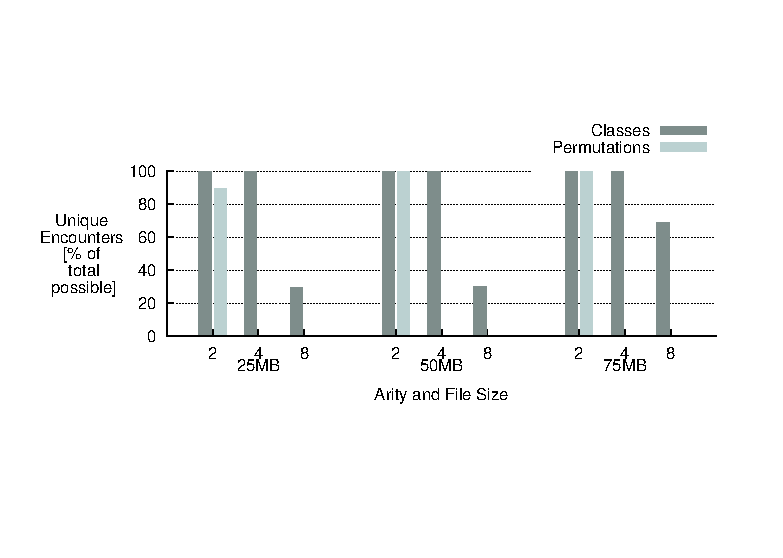
\includegraphics[width=2.5in]{experiments/sparse_english} &
\includegraphics[width=2.5in]{experiments/sparse_english_ints} \\ \\ \\
\mbox{DNA} & \mbox{Proteins} \\ 
\includegraphics[width=2.5in]{experiments/sparse_dna} &
\includegraphics[width=2.5in]{experiments/sparse_proteins} \\ \\ \\
\mbox{Sources} & \mbox{XML} \\
\includegraphics[width=2.5in]{experiments/sparse_sources} &
\includegraphics[width=2.5in]{experiments/sparse_dblp_xml}
\end{array}$
\end{center}
\caption{Sparsity measurements for each data file. The vertical axis represents
the percentage of \emph{total possible} classes and block permutations that were
witnessed for the given file size and arity when using the 
Multiary Wavelet Tree with Generalised RRR.}
\label{fig:sparse}
\end{figure}

\clearpage
		\DefFig[Uncompressed Multiary Wavelet Tree
			query times for English files]
			{fig:stime-eng}{experiments/simple_time_english}{0.9}
			{Query times for Uncompressed Multiary Wavelet Tree of increasing 
			arity for each \emph{English} file.}
		
		\DefFig[RRR Wavelet Tree query times for 75MB English file]
			{fig:time-eng-75}{experiments/time_english_75MB}{0.9}
			{Query times for RRR Wavelet Trees of increasing arity
			for the 75MB \emph{English} file.}
	
			\begin{figure}[h]
			\begin{center}
			$\begin{array}{cc}
			\mbox{(25MB English file)} & 
			\mbox{(50MB English file)} \\
			\includegraphics[width=2.5in]{experiments/time_english_25MB} &
			\includegraphics[width=2.5in]{experiments/time_english_50MB}
			\end{array}$
			\end{center}
			\caption{Query times for RRR Wavelet Trees of increasing arity
			for the 25MB and 50MB \emph{English} files.}
			\label{fig:time-eng-25-50}
			\end{figure}
			
From Figure \ref{fig:stime-eng} we can see how increasing the arity affects
querying a non-compressed Wavelet Tree. It is slower for increasing file size
because it is calculating rank queries without the assistance of RRR.

From Figures \ref{fig:time-eng-25-50} and \ref{fig:time-eng-75} we are able 
to see that increasing the file size does not significantly affect the time
performance of the Wavelet Trees which utilise RRR.

The Generalised RRR is slower than Claude's. We suspect that this is due to our 
use of pointers, as required to create a sparse table, whereas Claude's avoids 
dereferencing and may make better use of cache. The trend is similar to the
other Multiary Wavelet Trees, though.

The Multi-Binary RRR Wavelet Tree is faster than Claude's when the arity is 
increased. It is slower at arity 2 possibly due to optimisations in Claude's
Wavelet Tree code, or because we need to do an extra calculation to work out
the binary rank of all previous symbols (see Section 
\ref{sec:multi-bin-rrr}).

All other time graphs show similar trends, and so have been omitted\footnote{The 
other graphs are available at http://github.com/alexbowe/honours-thesis/}.

\clearpage
		\DefFig[Memory consumption for 75MB English file]
			{fig:mem-eng-75}{experiments/mem_english_75MB}{0.9}
			{Memory consumption for Wavelet Trees of increasing arity for
			the 75MB \emph{English} file. The size coefficient is a multiplier
			on the original file size. The bar stacked on top is the space for
			the supporting RRR table. The bar underneath is the space for
			the Wavelet Tree (which had negligible overhead) and each of its
			nodes, as RRR sequences or not. The Uncompressed Wavelet Tree is
			the only one which does not have a RRR table.}
		
		\begin{figure}[h]
		\begin{center}$
		\begin{array}{cc}
		\mbox{(25MB English file)} & 
		\mbox{(50MB English file)} \\
		\includegraphics[width=2.5in]{experiments/mem_english_25MB} &
		\includegraphics[width=2.5in]{experiments/mem_english_50MB}
		\end{array}$
		\end{center}
		\caption{Memory consumption for Wavelet Trees of increasing arity 
		for the 25MB and 50MB \emph{English} files.}
		\label{fig:mem-eng-25-50}
		\end{figure}

		\DefFig[Memory consumption for 75MB Words file]
			{fig:mem-words-75}{experiments/mem_english_ints_75MB}{0.9}
			{Memory consumption for Wavelet Trees of increasing arity for
			the 75MB \emph{Words} file. The size coefficient is a multiplier
			on the original file size. The bar stacked on top is the space for
			the supporting RRR table. The bar underneath is the space for
			the Wavelet Tree (which had negligible overhead) and each of its
			nodes, as RRR sequences or not. The Uncompressed Wavelet Tree is
			the only one which does not have a RRR table.}
		
			\begin{figure}[h]
			\begin{center}$
			\begin{array}{cc}
			\mbox{(25MB Words file)} & 
			\mbox{(50MB Words file)} \\
			\includegraphics[width=2.5in]{experiments/mem_english_ints_25MB} &
			\includegraphics[width=2.5in]{experiments/mem_english_ints_50MB}
			\end{array}$
			\end{center}
			\caption{Memory consumption for Wavelet Trees of increasing arity 
			for the 25MB and 50MB \emph{Words} files.}
			\label{fig:time-words-25-50}
			\end{figure}

Figure \ref{fig:mem-eng-75} shows how changing the arity affects the memory
consumption of the structures. We only show this for the 75MB file, as the 
others compress (or expand) with similar coefficients. Note that even though 
the generalised RRR structure's Wavelet Tree (which includes the RRR sequences 
it stores) is smaller than the original text, the size to contain the supporting 
RRR count structure is very large.

		\DefFig[Memory consumption for 75MB Proteins file]
			{fig:mem-prot-75}{experiments/mem_proteins_75MB}{0.9}
			{Memory consumption for Wavelet Trees of increasing arity for
			the 75MB \emph{Proteins} file. The size coefficient is a multiplier
			on the original file size. The bar stacked on top is the space for
			the supporting RRR table. The bar underneath is the space for
			the Wavelet Tree (which had negligible overhead) and each of its
			nodes, as RRR sequences or not. The Uncompressed Wavelet Tree is
			the only one which does not have a RRR table.}

		\begin{figure}[h]
		\begin{center}$
		\begin{array}{cc}
		\mbox{(25MB Proteins file)} & 
		\mbox{(50MB Proteins file)} \\
		\includegraphics[width=2.5in]{experiments/mem_proteins_25MB} &
		\includegraphics[width=2.5in]{experiments/mem_proteins_50MB}
		\end{array}$
		\end{center}
		\caption{Memory consumption for Wavelet Trees of increasing arity 
		for the 25MB and 50MB \emph{Proteins} files.}
		\label{fig:mem-prot-25-50}
		\end{figure}
		
The large size of the RRR Table for the Generalised RRR in Figure 
\ref{fig:mem-prot-75} appears to be the result of the large number of unique
permutations encountered for the Proteins file, since it has less classes but 
more permutations than the words file. See Tables .. and \ref{tab:maxclass}.
